

\documentclass[12pt]{article}
\usepackage{graphicx}
\usepackage{amsmath}
\usepackage{mathtools}
\usepackage{gensymb}

\newcommand{\mydet}[1]{\ensuremath{\begin{vmatrix}#1\end{vmatrix}}}
\providecommand{\brak}[1]{\ensuremath{\left(#1\right)}}
\providecommand{\norm}[1]{\left\lVert#1\right\rVert}
\newcommand{\solution}{\noindent \textbf{Solution: }}
\newcommand{\myvec}[1]{\ensuremath{\begin{pmatrix}#1\end{pmatrix}}}
\let\vec\mathbf

\begin{document}
\begin{center}
\textbf\large{CHAPTER-11 \\ CIRCLES}

\end{center}
\section*{Excercise 11.1}

Q10.Find the equation of the circle passing through the points $\brak{4,1} \text{ and } \brak{6,5}$ and whose centre is on the line $4x + y = 16$.

\solution
The equation of the circle is given by
\begin{align}
	\label{eq:circEq1}
	\norm{\vec{x}}^2 + 2\vec{x}^\top \vec{u} + f = 0
\end{align}
where
\begin{align}
	\vec{u} &= -\vec{c}\\
	      f &= \norm{\vec{c}} - r^2
\end{align}
Given points are
\begin{align}
	\label{eq:circPoints}
	\vec{x}_{1} = \myvec{4\\1} , \vec{x}_{2} = \myvec{6\\5}
\end{align}
And the line passing through the centre
\begin{align}
	\label{eq:line1}
	\myvec{4 & 1}\vec{x} = 16
\end{align}
Substituting points from \eqref{eq:circPoints} into \eqref{eq:circEq1}
\begin{align}
	\brak{4^2 + 1^2}+2\myvec{4 & 1}\vec{u}+f&=0\\
	\label{eq:eq1}	
	\implies 2\myvec{4 & 1}\vec{u}+f&=-17\\
	\brak{6^2 + 5^2}+2\myvec{6 & 5}\vec{u}+f&=0\\
	\label{eq:eq2}
	\implies 2\myvec{6 & 5}\vec{u}+f&=-61
\end{align}
And since \eqref{eq:line1} passes through the centre
\begin{align}
	-\vec{n}^\top \vec{u} &= c\\
	\label{eq:eq3}
	-\myvec{4 & 1}\vec{u} &= 16
\end{align}
Representing \eqref{eq:eq1},\eqref{eq:eq2} and \eqref{eq:eq3} in matrix form
\begin{align}
	\myvec{-4 & -1 & 0\\
	       12 & 10 & 1\\
	        8 &  2 & 1}
	\myvec{\vec{u}\\f} = 
	\myvec{16 \\ -61 \\ -17}
\end{align}
The augmented matrix is expressed as
\begin{align}
	\myvec{-4 & -1 & 0 & \vrule & 16\\
	       12 & 10 & 1 & \vrule & -61\\
	        8 &  2 & 1 & \vrule & -17}
\end{align}
Performing sequence of row operations to transform into an Echelon form
\begin{align}
	\xleftrightarrow[R_2\rightarrow R_2+3R_1]{{R_3\rightarrow R_3+2R_1}}
	\myvec{-4 & -1 & 0 & \vrule & 16\\
	        0 &  7 & 1 & \vrule & -13\\
	        0 &  0 & 1 & \vrule & 15}\\
	\xleftrightarrow[]{{R_2\rightarrow R_2-R_3}}
	\myvec{-4 & -1 & 0 & \vrule & 16\\
	        0 &  7 & 0 & \vrule & -28\\
	        0 &  0 & 1 & \vrule & 15}\\
	\xleftrightarrow[]{{R_2\rightarrow \frac{R_2}{7},R_1\rightarrow \frac{-R_1}{4}}}
	\myvec{ 1 & \frac{1}{4} & 0 & \vrule & -4\\
	        0 &  1 & 0 & \vrule & -4\\
	        0 &  0 & 1 & \vrule & 15}\\
	\label{eq:solution}	
	\xleftrightarrow[]{{R_1\rightarrow R_1-\frac{1}{4}R_2}}
	\myvec{ 1 &  0 & 0 & \vrule & -3\\
	        0 &  1 & 0 & \vrule & -4\\
	        0 &  0 & 1 & \vrule & 15}
\end{align}
So, from \eqref{eq:solution}
\begin{align}
	\vec{u} &= \myvec{-3\\-4}\\
	f &= 15 
\end{align}
Since $\vec{u} = -\vec{c}$
\begin{align}
	\vec{c} &= \myvec{3\\4}\\
	r^2 &= \brak{3^2+4^2} - 15\\
	r &= \sqrt{10}
\end{align}
Hence, the equation of circle is
\begin{align}
	\norm{\vec{x}}^2 +2\vec{u}^\top \vec{x}+15 = 0\\
	\text{ where } \vec{u} = \myvec{-3\\-4}
\end{align}
The corresponding is shown in Figure \ref{fig:Fig1}
\begin{figure}[!h]
	\begin{center} 
	    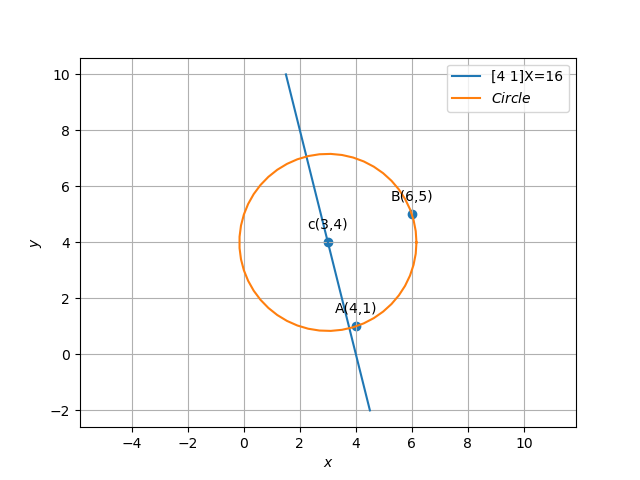
\includegraphics[width=\columnwidth]{figs/circ2}
	\end{center}
\caption{}
\label{fig:Fig1}
\end{figure}





\end{document}
